\PassOptionsToPackage{full}{textcomp}
\documentclass[]{tufte-handout}
%\usepackage{fontspec}

% load babel package and options here
%\usepackage[p,osf]{ETbb} % osf in text, tabular lining figures in math
\usepackage{ETbb} % osf in text, tabular lining figures in math
\usepackage[scaled=.95,type1]{cabin} % sans serif in style of Gill Sans
\usepackage[varqu,varl]{zi4}% inconsolata typewriter
\usepackage[T1]{fontenc} % LY1 also works
\usepackage[libertine,vvarbb]{newtxmath}
%\usepackage[cal=boondoxo,bb=boondox,frak=boondox]{mathalfa}

%\geometry{showframe} % display margins for debugging page layout

\usepackage{graphicx} % allow embedded images
%  \setkeys{Gin}{width=\linewidth,totalheight=\textheight,keepaspectratio}
  \graphicspath{{graphics/}} % set of paths to search for images
\usepackage{amsmath}  % extended mathematics
\usepackage{booktabs} % book-quality tables
%\usepackage{units}    % non-stacked fractions and better unit spacing
\usepackage{multicol} % multiple column layout facilities
\usepackage{lipsum}   % filler text
\usepackage{fancyvrb} % extended verbatim environments
  \fvset{fontsize=\normalsize}% default font size for fancy-verbatim environments
\usepackage{gensymb} % provides symbols like \degree
\usepackage{ragged2e} % enables hyphenation in ragged-right justification
\usepackage[normalize-symbols]{textalpha} %enables \textalpha for alpha symbol etc.

\usepackage{hyperref} % enables styling of href and url
\hypersetup{
    pdftitle={Mechanisms},
    pdfauthor={Barry Linkletter},
    colorlinks=true,
    linkcolor=blue,
    filecolor=magenta,      
    urlcolor=blue,
    pdfborder={0 0 0},
    frenchlinks=false,
    pdfpagemode=FullScreen,
    }
    \urlstyle{same}
\makeatletter
% Inspired by http://anti.teamidiot.de/nei/2009/09/latex_url_slash_spacingkerning/
% but slightly less kern and shorter underscore
\let\UrlSpecialsOld\UrlSpecials
\def\UrlSpecials{\UrlSpecialsOld\do\/{\Url@slash}\do\_{\Url@underscore}}%
\def\Url@slash{\@ifnextchar/{\kern-.03em\mathchar47\kern-.15em}%
    {\kern-.0em\mathchar47\kern-.08em\penalty\UrlBigBreakPenalty}}
\def\Url@underscore{\nfss@text{\leavevmode \kern.06em\vbox{\hrule\@width.3em}}}
\makeatother

\usepackage{enumitem} % allows resuming enumerate lists.
\usepackage{mathtools}
\usepackage{mhchem}

\usepackage{siunitx} % provides "S" column class for aligning decimals.  
         \sisetup{uncertainty-mode = separate}

\usepackage{nicefrac}

\usepackage[nospace]{varioref}
    \renewcommand\reftextfaceafter{on the following page}
    \renewcommand\reftextafter {on the next page}
    \renewcommand\reftextfacebefore{on the previous page}
    \renewcommand\reftextbefore {on the previous page}

\newcommand{\tss}[1]{\textsuperscript{#1}}

\usepackage[english]{babel}
\usepackage{float}
\usepackage{stackrel}

\usepackage[shortconst]{physconst}

\usepackage[normalem]{ulem}  % provides strikethrough \sout{}

\usepackage{newfloat}
\DeclareFloatingEnvironment[
  fileext = los ,
  listname = {List of Schemes} ,
  name = Scheme
]{scheme}

\usepackage{newfloat}
\DeclareFloatingEnvironment[
  fileext = loe ,
  listname = {List of Eqs} ,
  name = Equation
]{equate}

\usepackage{listings}

%%%%%%%%%%%%%%%%%%%%%%%%%%%%%%%%%%%%%%%%%%%%%%%%%%%%%%%%%%%

\title{Interpolating Literature Data Sets}
\author[Barry Linkletter]{Barry Linkletter}
\date{} % without \date command, current date is supplied


\begin{document}

\justifying

\maketitle
\marginnote[-15mm]{This document was produced using the \LaTeX\ typesetting language with the Tufte-handout document class. Chemical diagrams were created in \textit{ChemDoodle} and calculations and plotting were performed using \textit{Python} tools in a \textit{Jupyter Notebook}. Diagrams and plots were further edited in \textit{Affinity Designer}\vspace{3mm}}
%\justify
\begin{abstract}

\noindent Many data sets in the literature list values such as $H_0$ or activity coefficients for mixtures of acids (and other solvent conditions). However they may not have a data point exactly where you need it to be. To extract the information that you want you will need to interpolate.

\end{abstract}




\section{Hunting for Data}


I have a system where rate constants of a reaction, $k_{obs}$, in various sulphuric acid mixtures have been reported. I am constructing a plot that will relate the activity of water, $a_{\ce{H2O}}$, the acidity function to the mixture, $H_0$, to this rate constant. I need values for $a_{\ce{H2O}}$ and $H_0$ for the mixtures used in the experiment. Fortunately, the chemical literature has many examples of such tables, and a few have become the standards in the field. Table~\ref{tab:tab1} below lists some data sources that might be useful for our investigation.

\begin{table}[h!]
\centering
\caption[][-40mm]{Chemical data for properties of mixtures of sulphuric acid. \\ $\longleftarrow$ \\ \vspace{2mm}References are listed below\ldots \vspace{2mm}

\noindent J.A. Rard et al., \textit{J. Chem. Engin. Data}, \textbf{1976}, \textit{21}, 374-379. \url{https://doi.org/10.1021/je60070a002} \vspace{1mm}

\noindent W.F. Giauque et al., \textit{J. Am. Chem. Soc.}, \textbf{1960}, \textit{82}, 62-70. \url{https://doi.org/10.1021/ja01486a014} \vspace{1mm}

\noindent H. Yang al., \textit{J. Solution Chem.}, \textbf{2016}, \textit{45}, 1580–1587. \url{https://doi.org/10.1007/s10953-016-0516-4} \vspace{1mm}

\noindent C.D. Johnson et al., \textit{J. Am. Chem. Soc.}, \textbf{1969}, \textit{91}, 6654-6662. \url{https://doi.org/110.1021/ja01052a021} \vspace{1mm}

\noindent P. Tickle et al., \textit{J. Chem. Soc. B}, \textbf{1970}, 65-70 \url{https://doi.org/10.1039/J29700000065} \vspace{1mm}

\noindent M.J. Jorgenson, D.R. Hartter, \textit{J. Am. Chem. Soc.}, \textbf{1963}, \textit{85}, 878-883. \url{https://doi.org/10.1021/ja00890a009} \vspace{1mm}

\noindent R.J. Gillespie et al., \textit{J. Am. Chem. Soc.}, \textbf{1971}, \textit{93}, 5083-5087. \url{https://doi.org/10.1021/ja00749a021} \vspace{1mm}

\noindent J. Sierra et al,, \textit{J. Chem. Soc. B}, \textbf{1970}, 1570-1573. \url{https://doi.org/10.1039/J29700001570} \vspace{1mm}

\noindent E. H{\"o}gfeldt,  J. Bigeleisen, \textit{J. Am. Chem. Soc.}, \textbf{1960}, \textit{82}, 15-20. \url{https://doi.org/10.1021/ja01486a005} \vspace{1mm}

\noindent M.J. Cook et al., \textit{J. Am. Chem. Soc.}, \textbf{1975}, \textit{97}, 760-764. \url{https://doi.org/10.1021/ja00837a012} \vspace{1mm}

\noindent N.C. Deno et al., \textit{J. Am. Chem. Soc.}, \textbf{1955}, \textit{57}, 3044-3051. \url{https://doi.org/10.1021/ja01616a036} \vspace{1mm}

\noindent CRC Handbook of Chemistry and Physics, 106\textsuperscript{th} ed. \textbf{2025}, J.R. Rumble, ed., \textit{CRC Press, Taylor \& Francis, Boca Raton, FL}. \url{https://library.upei.ca/chem} or get the \href{https://hbcp-chemnetbase-com.proxy.library.upei.ca/documents/05_29/05_29_0081.xhtml?dswid=9598}{PDF  here} or \href{https://hbcp-chemnetbase-com.proxy.library.upei.ca/contents/ArchiveSearch.xhtml?dswid=9598\&faces-redirect=true\#}{here}.
}
\label{tab:tab1}
    \begin{tabular}{cll}
%        \toprule
        {Data} & {\ce{H2SO4} Mixture}     & {Source} \\
        \midrule
           $a_{\ce{H2O}}$  & $1$ to \qty{75}{\%}  &   Rard, 1976   \\
           $a_{\ce{H2O}}$  & $9$ to \qty{99}{\%}  &   Giauque, 1960    \\
           $a_{\ce{H2O}}$  & $20$ to \qty{42}{\%} &   Yang, 2016    \\
           $H_0$           & $1$ to \qty{60}{\%}  &   Johnson, 1969    \\
           $H_0$           & $4$ to \qty{98}{\%}  &   Tickle, 1970    \\
           $H_0$           & $60$ to \qty{99}{\%}  &   Jorgenson, 1963    \\
           $H_0$           & $98$ to \qty{100}{\%}  &   Gillespie, 1971    \\
           $D_0$           & $8$ to \qty{99.6}{\%}  &   Sierra, 1970    \\
      $H_0$ \& $D_0$       & $10^{-3.8}$ to \qty{1}{\mole \per \litre}  &   H{\"o}gfeldt, 1960    \\
           $H_R$           & $6$ to \qty{90}{\%}  &   Cook, 1975    \\
           $H_R$           & $0.5$ to \qty{98}{\%}  &   Deno, 1955    \\
           $density$       & $0.5$ to \qty{100}{\%}  &   CRC Handbook    \\
%        \bottomrule
    \end{tabular}
\end{table}

\vspace{1em}


There are many options for a particular property in a given acid mixture. Hopefully, they all agree. Spoiler alert: they sometimes do not. However, subsequent publications will reveal the data sets most accepted by the field. So, do not grab just any data set; read widely and get a sense of which is most trusted. Over time, even well-respected groups have their data cast aside as more modern methods reveal better measurements.

\newpage
\section{The Land of In-Between}

When analyzing literature results, we sometimes find it informative to replot published data against more modern data sets and see if we reach the same conclusions as the authors (a \qty{100}{\percent} success rate so far). In the analysis that we are currently engaged in, I will need to obtain data for the activity of acid ($h_0$), the activity of water ($a_{\ce{H2O}}$) and the molar concentration of water (will require the density of the mixture) in given mixtures of sulphuric acid and water. 

We are investigating the observed rate constant for methyl acetate hydrolysis in concentrated sulphuric acid mixtures.\sidenote[][-10mm]
{"Mechanisms of ester hydrolysis in aqueous sulfuric acids."
K. Yates, R.A. McClelland,
\textit{J. Am. Chem. Soc.}, \textbf{1967}, \textit{89}, 2686-2692.
\url{https://doi.org/10.1021/ja00987a033} \label{ref:ref1}}
 I will use the data set from The data from the paper Giauqueet (1960) for $a_{\ce{H2O}}$, the data from Tickle (1970) for  $H_0$ (We can calculate $h_0$ from $H_0$), and the density data from the CRC Handbook (from which we can calculate $[\ce{H2O}]$.)\sidenote[][0mm]{The references are given in table~\ref{tab:tab1}} 
 
Table~\vref {tab:tab2} presents data from all my sources. You can see that the data points for the various values seldom line up. How will I obtain a literature value for  $H_0$, $a_{\ce{H2O}}$ and density at the experimental concentrations used in the rate study?\textsuperscript{\ref{ref:ref1}} The answer is to interpolate values between the data points of the literature data sets.

I could use an interpolation function that provides values on straight lines between each data point. This linear interpolation method will deliver excellent results with most data sets. A slightly better method is to use a Blpline interpolation to give me values on a curving spline between data points. This is useful if the data has a smooth curve and significant spacing between points. When using a spline, one must ensure that we are not getting a wiggle between data points as it attempts to run the spline through each point. I chose to use a smoothing Bspline function provided by the \textit{SciPy.Interpolate} library in \textit{Python}.\sidenote[][0mm]{See the interactive \textit{Python} notebooks on Google Colab.} This function will create a smooth interpolation on a spline, but it is not mathematically required to pass through each data point. It is suitable for moderately noisy data. Our data sets are produced by authors who reported the values based on polynomial curve fits through their own experimental data and are noise-free. We do not have access to the underlying data and only have the data points reported in each publication. So we will interpolate.


\begin{table}[h!]
\centering
\caption{Pseudo-first order rate constants for hydrolysis of methyl acetate at \qty{25}{\degreeCelsius}.\textsuperscript{\ref{ref:ref1}} Selected data for $H_0$, $a_{\ce{H2O}}$ and density are included. Observe that we do not have exact matches between the reaction conditions reported and the values for our literature data.\\ $\longleftarrow$ \\
\vspace{40mm}
For example: Observe that we have a rate reported at \qty{45.4}{\percent} \ce{H2SO4}. We have data for $H_0$ for \qty{44}{\percent}  and \qty{50}{\percent}  mixtures, but not at \qty{45.4}{\percent}.  Data for water activity is not available for \qty{50}{\percent}  but is at \qty{51.9}{\percent}. How shall we find values in the spaces between data points in literature tables? The answer is interpolation. \\ $\longleftarrow$
}
\label{tab:tab2}
    \begin{tabular}{SSSSS}
%        \toprule
        {$\%\ce{H2SO4}$}      & {$k_{obs}/\qty{e{-2}}{min^{-1}}$} & {$H_0$}   & {$a_{\ce{H2O}} / \num{e{-2}}$} & {$\rho / \unit{\g \per \cm \cubed}$} \\
        \midrule
          8.9               &                                  &               &   96.22      &             1.0947      \\
        14.1               &   1.50                        & -0.59      &             {}   &               {}         \\
        20                  &                                  & -0.99      &                  &             1.1398      \\
        20.7               &   2.61                        &            {} &            {}    &               {}          \\
        22.7               &                                  &               &  85.14        &                         \\
        22                  &                                  & -1.13      &                   &             1.1554      \\
        28.3               &   4.22                        &            {} &   78.00       &              {}          \\
        30                  &                                  & -1.63      &                   &             1.2191      \\
        32.9               &                                  &               &   70.35       &                         \\
        34.8               &   6.41                        &            {} &            {}    &             {}           \\
        36                  &                                  & -2.09      &                   &             1.2685      \\
        37.0               &                                  &               &   62.57       &                         \\
        40.4               &   8.14                        &           {} &            {}     &              {}           \\
  	40.7              &                                   &              &  55.03         &                         \\
        44                 &                                   & -2.69     &  48.06         &             1.3386      \\
        45.4              &  10.4                          &           {} &            {}      &             {}           \\
        50                 &                                   & -3.21     &                     &             1.3952      \\
        51.9              &                                   &              &   31.13         &                         \\
        50.2              &  11.4                          &           {} &            {}      &             {}            \\
        54                 &                                   & -3.65     &   26.78         &             1.4351      \\
        55.2              &  13.3                          &           {} &            {}      &            {}             \\
        58                 &                                   & -4.10     &   19.80         &             1.4770      \\
        60.4              &  13.8                          &           {} &             {}     &             {}           \\
        64                 &                                   &  -4.85    &  10.77          &                         \\
        65.2              &  11.9                          &           {} &             {}     &             {}            \\
        66                 &                                   &  -5.10    &   7.929        &                         \\
        70                 &                                   &  -5.68    &                    &             1.6105      \\
        70.4              &   7.25                         &           {} &            {}      &              {}          \\
        71.0              &                                   &              &   3.799         &                         \\
       74                  &                                   &  -6.24    &                    &                         \\
       74.1               &   3.83                         &           {} &             {}    &             {}          \\
       79.7               &                                   &              &  0.590         &                         \\
       80.0               &   0.931                       &  -7.17    &            {}     &          1.7272         \\
       81.5               &                                   &              &  0.353         &                         \\

%        \bottomrule
    \end{tabular}
\end{table}



\section{The Tools for Interpolation}

I have written short blobs of \textit{Python} code that will read in a data file and create an interpolation function based on that data. Once the interpolation function is created it will return a \textit{y}-value when given an \textit{x}-value. The result should give a very good estimate for values between points of our data set. Since I am using a smoothing interpolation function, the results at each data point where we have a known \textit{x},\textit{y} pair may differ slightly. This will be due the precision of the numbers (most values have only three significant figures) and also slight drift at the ends of the data sets where the spline-creating math will have less data to work with.

In figures~\ref{fig:fig1}, \ref{fig:fig2} and \vref{fig:fig3} present the data sets chosen for this project with the Bspline interpolation plotted as well.\sidenote[][0mm]{The \textit{Python} notebook for the plots in Figures~\ref{fig:fig1}, \ref{fig:fig2} and \vref{fig:fig3} above can accessed via Google Colab at \url{https://colab.research.google.com/github/blinkletter/4410PythonNotebooks/blob/main/Class_30/Yates-interpolators.ipynb}} With each plot there will also be presented the calculated residuals at the known data points.  You can see that the spline interpolation tracks with the data within a few tenths of a percent in most cases. You can change how closely the spline tracks the data points by editing the \textit{Python} code.


\begin{figure*}[h!]
  \centering
  \caption[][-0mm]{Data and interpolation of the $a_{\ce{H2O}}$ data from Giauqueet, 1960. $\uparrow$} 
  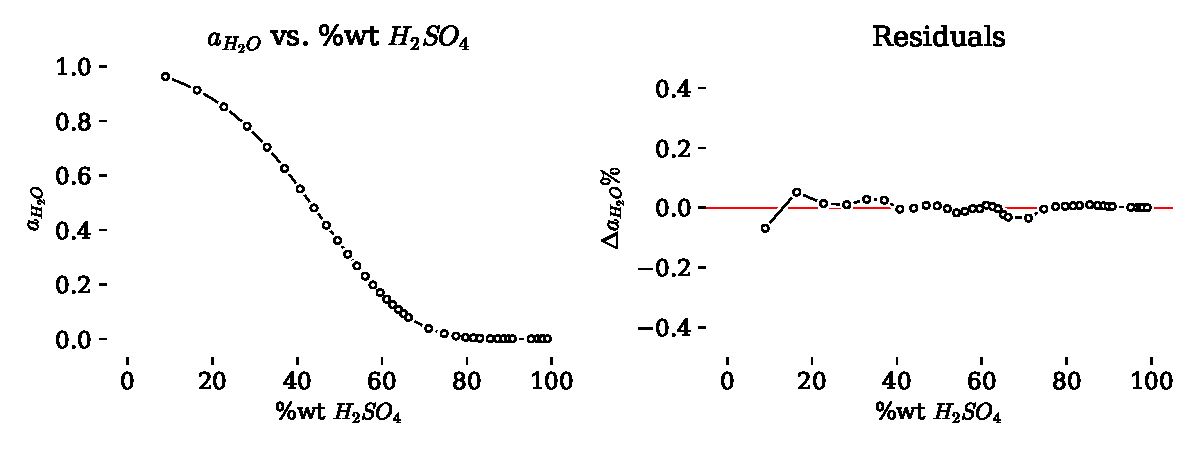
\includegraphics[scale=0.7]{images/aH2O_interp}
  \label{fig:fig1}
\end{figure*}

\begin{figure*}[h!]
  \centering
  \caption[][-0mm]{Data and interpolation of the $H_0$ data from Tickle, 1970. $\uparrow$} 
  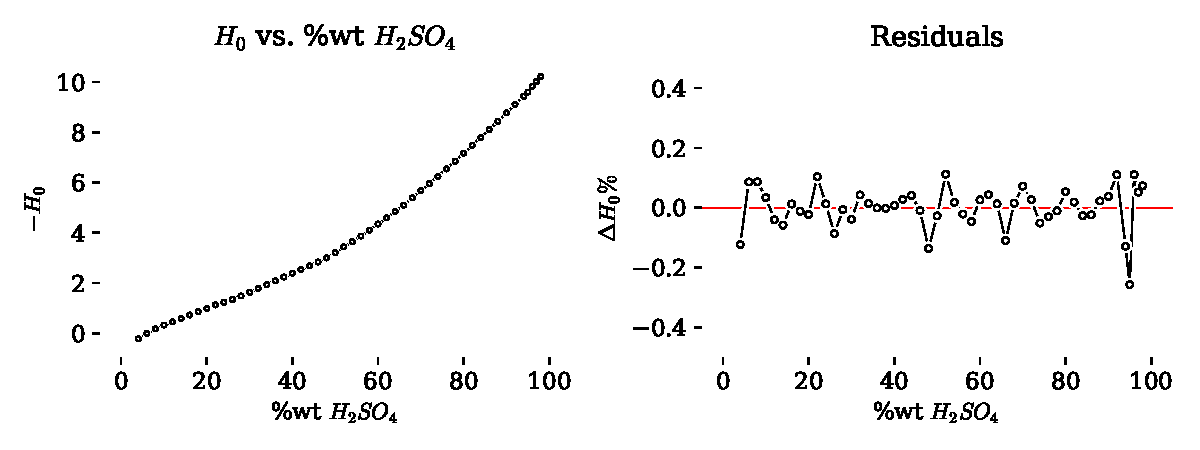
\includegraphics[scale=0.7]{images/H0_interp}
  \label{fig:fig2}
\end{figure*}


\begin{figure*}[h!]
  \centering
  \caption[][-0mm]{Data and interpolation of the density data from the CRC handbook, 2023. $\uparrow$} 
  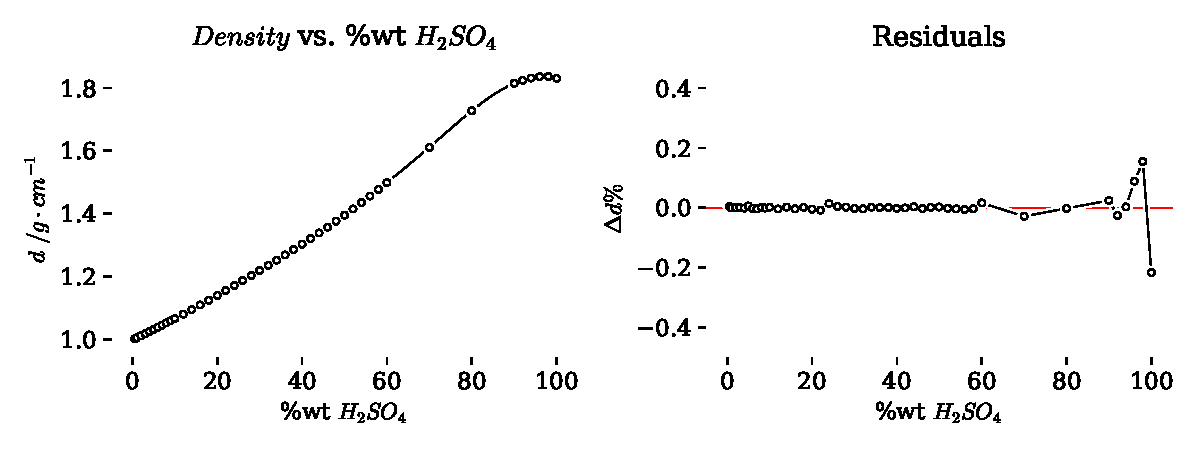
\includegraphics[scale=0.7]{images/Density_interp}
  \label{fig:fig3}
\end{figure*}

\clearpage

\section{Applying the Interpolations}

By applying the three interpolation functions at the values for \%\ce{H2SO4} in the data table for rates of hydrolysis\textsuperscript{\ref{ref:ref1}} we can estimate values for $H_0$, $a_{\ce{H2O}}$ and density. The results of this are presented in table~\ref{tab:tab3}.

\begin{table}[h!]
\centering
\caption{Pseudo-first order rate constants for hydrolysis of methyl acetate at \qty{25}{\degreeCelsius}.\textsuperscript{\ref{ref:ref1}} Interpolated data for $H_0$, $a_{\ce{H2O}}$ and density are included. Only five data points matched up in the tables against the concentrations used by the authors. All other values for $H_0$, $a_{\ce{H2O}}$ and density were estimated by interpolation.\\ $\longleftarrow$ \vspace{2mm}}
\label{tab:tab3}
    \begin{tabular}{SSSSS}
%        \toprule
        {$\%\ce{H2SO4}$}      & {$k_{obs} / \qty{e{-2}}{min^{-1}}$} & {$H_0$}   & {$a_{\ce{H2O}} / \num{e{-2}}$} & {$\rho / \unit{\g \per \cm \cubed}$} \\
        \midrule
           14.1               &   1.50        & -0.59    &  93.0          & 1.095  \\
           20.7               &   2.61        &  -1.04            &  87.4          &  1.145         \\
           28.3               &   4.22        &  -1.51            & 78.0  &  1.205         \\
           34.8               &   6.41        &  -2.00            &  66.9          &  1.258         \\
           40.4               &   8.14        &  -2.42            &  55.7          &  1.306         \\
           45.4               &  10.4         &  -2.79            &  45.0          &  1.351         \\
           50.2               &  11.4         &  -3.23            &  34.7          &  1.397         \\
           55.2               &  13.3         &  -3.78            &  24.6          &  1.448         \\
           60.4               &  13.8         &  -4.40            &  15.6          &  1.503         \\
           65.2               &  11.9         &  -5.00            &   9.09         &  1.556         \\
           70.4               &   7.25        &  -5.74            &   4.23         &  1.615         \\
           74.1               &   3.83        &  -6.26            &   2.157        &  1.659         \\
           80.0               &   0.931       & -7.17    &   0.538        & 1.727  \\

%        \bottomrule
    \end{tabular}
\end{table}
\vspace{5mm}
We now have all the data necessary to construct the plot of the model for the $A_{Ac}2$ acid-catalyzed ester hydrolysis in concentrated acidic conditions.


\end{document}
